\chapter{Preliminary Vocabulary}
\label{vocab}

Before we start, there are a few uncommon terms we will use fairly often in this paper. We have briefly defined them here.

\section{Mondegreens}
\label{vocab:mondegreens}

A mondegreen is a word or phrase resulting from a misinterpretation of a word or phrase that has been heard\cite{dictionaryDotComMondegreen}.  The word was coined by American author Sylvia Wright in her article, ``The Death of Lady Mondegreen", published in a 1954 issue of Harper's Bazaar. In it, she describes the origin of the word:
\begin{quote}
When I was a child, my mother used to read aloud to me from Percy's Reliques, and one of my favorite poems began, as I remember:
    \begin{verse}
    Ye Highlands and ye Lowlands, \\
    Oh, where hae ye been? \\
    They hae slain the Earl O' Moray,\\
    And Lady \emph{Mondegreen.}
    \end{verse}
}
\end{quote} 
The fourth line of the quote is actually ``and laid him on the green"\cite{mondegreenOriginRef}.  

Additional commonly-cited mondegreens include\cite{gladlyTheCrossRef}\cite{purpleHazeRef}\cite{badMoonRisingRef}:
\begin{center}
\begin{tabular}{cc}
 Gladly the Cross-Eyed Bear & Gladly the Cross I'd Bear  \\
 Scuse me while I kiss this guy & Scuse me while I kiss the sky  \\
 There's a bathroom on the right & There's a bad moon on the rise  \\
\end{tabular}
\end{center}


\section{Oronyms}
\label{vocab:oronyms}

Oronyms are phrases that may differ in meaning or spelling, but  sound near-identical when spoken.  They are similar to mondegreens, and the terms are often used interchangeably.  The difference, however, lies in the context.  The label ``mondegreen" is used more often in regards to music lyrics, where pronunciation can be affected by the addition of music and tone to the phrase. Oronyms, on the other hand, refer to spoken words, not sung lyrics.\cite{dictionaryOronymDef}

Common oronyms include:
\begin{center}
\begin{tabular}{ cc }
i scream & ice cream \\
an ice cold hour & a nice cold hour \\
grape ants & gray pants \\
real eyes & realize \\
\end{tabular}
\end{center}

\section{Orthography}
\label{vocab:orthography}
The word `orthographic' comes from the Latin \emph{orthographia}, meaning \emph{correct} writing.   Orthography itself is the part of language study concerned with letters and spelling.  More specifically, it's the standardized system of writing down words in a specific language, using a commonly-accepted set of letters according to accepted usage. \cite{dictionaryDotComOrthography} 

The orthographic symbol set for a language is the commonly-accepted set of letters used to spell words in that language.  In English, our orthographic symbol set is the Latin alphabet.

In this paper, ``orthographic phrase'', refers to a sequence of regularly-spelled words found in an English dictionary.

\begin{figure}[h]
\begin{center}
Example:  
\fbox{
\textquotedblleft This is a orthographic phrase.\textquotedblright
}
\end{center}
\end{figure}


\section{Phonetics and Phonology}
\label{vocab:phoneticsAndPhonology}
To discover oronyms for a phrase, we must first to translate the root orthographic phrase to a representation that allows us to unambiguously measure pronunciation.   Phonology and phonetics are branches of linguistics that deal with pronunciation.

\subsection{Phonetics}
\label{vocab:phonetics}
Phonetics is a branch of \emph{descriptive} linguistics, and refers to the study of the actual, uttered sound of human speech. It deals with describing the physical phenomena of how these sounds are produced from the vocal tract, how they are transmitted once spoken, and how they are recieved by audiences. The building blocks of phonetics are \emph{phones}, which represent atomic sounds.

\subsection{Phonology (aka phonemics)}
\label{vocab:phonology}
Phonology is a branch of \emph{theoretical} linguistics, and as such, is primarily concered with the abstract grammartical characterization of sounds.  It describes the way that sounds function within a language and give meaning to words.  The basis of phonological analysis is the grouping of sounds (\emph{phones}) into distinct units within a languages.  These distinct units are called \emph{phonemes}.  

These phonemes may contain different phones, depending on the accent of the speaker.  For example, native speakers of General American English only generally recognize one `L' sound phoneme. However, there are two different ways that that phoneme manifests itself: the `l' in ``male", and the `l' in late. This difference is not noticable to a native speaker of American English, because that particular accent will parse any `L' phone as the same `L' phoneme.

\subsection{Phonetics Vs Phonology}
\label{vocab:phoneticsVsPhonemics}

As we said previously, though the terms are sometimes used interchangably, the words `phonemic' and `phonetic' (and their corresponding sound building blocks, `phone' and `phoneme')  indicate a different stages of sound parsing.  \emph{Phonemes} are idealized sounds; \emph{phones} are the actual sounds that come out of a person's mouth.  Figure ~\ref{fig:knightsPhoneticPhonemic} provides a final, illustrative metaphor of the difference.
%\begin{center}
\begin{figure}[b]
\centering
        \begin{subfigure}[b]{0.4\textwidth}
                \centering
                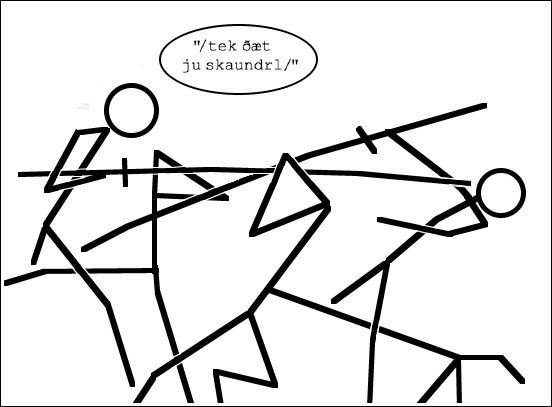
\includegraphics[width=\textwidth]{knights_phonemic.jpg}
                \captionfonts
                \caption[Phonemic Knights]{Phonology\cite{cartoonPhonemic} }
                \label{fig:cartoonPhonemic}
        \end{subfigure}
        \quad
        \begin{subfigure}[b]{0.4\textwidth}
                \centering
                
\includegraphics[width=\textwidth]{knights_phonetic.jpg}
                \captionfonts
                \caption[Phonetic Knights]{Phonetics\cite{cartoonPhonetic} }
                \label{fig:cartoonPhonetic}
        \end{subfigure}
\caption{The difference between phonetics and phonology}\label{fig:knightsPhoneticPhonemic}
\end{figure}
%\end{center}    

\FloatBarrier

\section{Phonemic/Phonetic Alphabets}
\label{section:phonemicAlphabets}
\begin{wrapfigure}{r}{0.5\textwidth}
\begin{center}
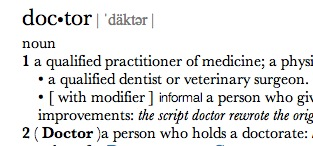
\includegraphics[width=70mm]{doctorDictIPAScreenshot.jpg}
\captionfonts
\caption[Dictionary IPA screenshot]{ The characters to the right of the large bold word ``doctor" are IPA symbols. }
\label{fig:doctorDictIPAScreenshot}
\end{center}
\end{wrapfigure}

As we stated in section ~\ref{vocab:phonology}, phonemes are the atomic building blocks of words. In a phonemic alphabet, every meaningful sound has its own letter.  The way that we interact with phonemes in a concrete way is by using phonetic alphabets and phonetic dictionaries.  


The most common phonetic alphabet is the IPA (Internation Phonetic Alphabet). It contains representations of every sound in every known language globally, and allows for cross-cultural pronunciation guidelines.  As shown in figure ~\ref{fig:doctorDictIPAScreenshot}, IPA representations of orthographic words are found in traditional dictionaries to aid pronunciation. 

\subsection{SAMPA}
\label{section:sampaAlphabet}

SAMPA (Speech Assessment Methods Phonetic Alphabet) is a computer-readable phonetic alphabet, based upon the symbols found in the more-standard-but-not-easily-computer-readable  IPA (International Phonetic Alphabet).  
It uses ``letters" consisting of 1-2 ASCII characters to represent each phoneme. The ASCII sequences for the SAMPA letter are designed so that any SAMPA sequence is deterministically parsible.

We chose to use SAMPA instead of IPA because its ASCII-compliance makes it easy to integrate into other systems.

See table ~\ref{table:sampaTable} for a full table of each SAMPA phoneme, its description, and its sub-parts.

For some brief context, the SAMPA spelling of the name `Jenee Hughes' is \emph{dZEni hjuz}.  
`Dr Zoe Wood'  becomes \emph{dAkt@\char18r zoui wUd}.  
`Dr John Clements' becomes \emph{dAkt@\char18r dZAn klEm@nts}. 
`Dr Franz Kurfess' becomes \emph{dAk@\char18r fr\{nz k3\char18rfEs}.



